\section{Data Understanding}

The task involved exploring the two assigned datasets: \texttt{cyclists.csv}, containing information about the cyclists, and \texttt{races.csv}, which includes race results and race-related data over the years. This provided an overall understanding of the data, which was useful for subsequent analysis and modeling tasks.

% -------------- cyclists dataset ------------------
\subsection{Cyclists Dataset}
\textbf{Dataset Overview and Key Insights}\\
The dataset consists of $6'134$ rows, each representing a specific cyclist. Each cyclist is identified by a unique \textit{\_url} and described by the following features: \textit{name}, \textit{birth\_year}, \textit{weight}, \textit{height}, and \textit{nationality}. The cyclists in the dataset have birth years ranging from 1933 to 2004. Based on the distribution, 75\% of the cyclists were born from 1962 onward, while only 25\% were born before 1962 (first quartile), indicating a much higher representation of cyclists born in more recent decades. \\
The \textit{height} and \textit{weight} of cyclists follow approximately a bell-shaped distribution. In particular, most cyclists have a height centered around 180 cm and a weight of around 70 kg. This suggests that cyclists tend to have a “standard” physique, with height and weight values centered around those values. \\
We can state that 86.50\% of cyclists are from Europe, and in particular, 57\% of the dataset consists of cyclists from only 4 European nations: Italy (the country with the most cyclists), Spain, Belgium, and France.\\
In terms of \textbf{feature correlations}, the only notable relationship observed is between \textit{height} and \textit{weight}, which aligns with expectations that taller cyclists generally weigh more.\\

\noindent
\textbf{Null Values and Outliers}\\  
The features \textit{\_url} and \textit{name} have 0 null values, \textit{nationality} has only 1 null value, \textit{birth\_year} has 13 null values, while \textit{weight} and \textit{height} have many null values, with half of the values missing for both. The null values are observable in \autoref{fig:null_values}. Excluding \textit{birth\_year}, all other numerical features exhibit outliers that follow either a symmetric distribution or are slightly skewed, as shown in the box plots presented in the notebook.\\

\noindent
\textbf{Consistency}\\
There are duplicate cyclist names, but no duplicate URLs. As we show in the notebook, usually the same name is associated with different cyclists which can be discriminated by a different URL and other feature values, if available.\\

\begin{figure}[H]
    \centering
    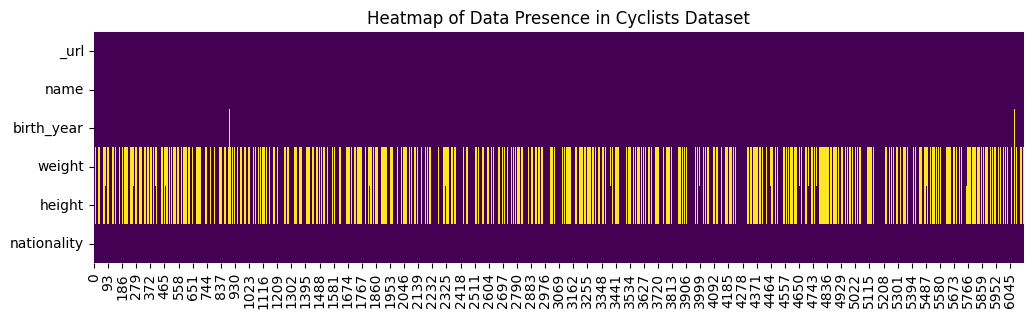
\includegraphics[width=0.7\linewidth]{images//DU/null_values.png}
    \caption{\small Null value heat-map in cyclists dataset}
    \label{fig:null_values}
\end{figure}

% -------------- Races dataset ------------------

\subsection{Races Dataset}

The dataset contains over $589'865$ rows, organized by race and stage. Each race, such as the "Giro d'Italia", is represented by multiple stages, and each stage is identified by a unique \textit{\_url}. The dataset includes several rows for each cyclist participating in the same stage, leading to the repetition of stage-related information. Additional features capture cyclist-specific details, including their identity, age, and team affiliation. 

\subsubsection{Feature overview}


\noindent \textbf{\_url}: this categorical alphanumeric column contains the unique URL identifier for each race stage and is repeated for every cyclist participating in that stage. \\

\noindent \textbf{name}:
This categorical alphanumeric column represents the race name for each stage, with 27 unique race names in the dataset. Variations in names arise from minor differences in spelling, accents, or naming conventions over time. For instance, \enquote{san-sebastian} corresponds to names like \enquote{Clasica Ciclista San Sebastian}, \enquote{Clásica Ciclista San Sebastián}, and \enquote{Clásica San Sebastián}, all referring to the same race.\\ 

\noindent \textbf{points}: 
This numerical attribute represents points assigned by the race, which can be the same for multiple cyclists. There are 4 stages with null values, resulting in a total of 477 null rows, but there are no illegal values (such as negative numbers, extreme outliers, or inconsistent values for the same stage). The points range from 50 to 150, with 50 being the most frequent value. The average is 89, and the median is 80.
On average, we can notice that the average point values are decreasing over the years.\\ 

\noindent \textbf{uci\_points}: This feature is similar to the previous one, but the points here are the official ones assigned by the UCI organ. There are $3'862$ stages with missing values, totaling $338'779$ rows in the dataset. The values range from 6 to 800, with the most frequent values being 100, 6, and 60. The mean is 82, and the median is 60.\\

\noindent \textbf{length}: this feature represents the total stage length in meters, with values ranging from 1 km to 338 km and a mean of 166 km. There are no null or inconsistent values in this feature, and the distribution exhibits two peaks: one for very short races and another for longer races. \\

\noindent \textbf{climb\_total}: this feature represents the total elevation gain of the stage in meters, with values ranging from 2 m to $6'974$ m and a mean of $2'375$ m. There are $2'214$ stages with null values, totaling $147'045$ rows, but no inconsistent values. The distribution shows two peaks: one for stages with minimal elevation gain and another for stages with higher elevation gains. This reinforces the idea mentioned earlier: there are primarily two types of races, shorter ones and longer ones.\\

\noindent \textbf{profile}: this categorical feature represents the race profile, with increasing difficulty levels ranging from 1 to 5, corresponding to: flat, hilly, mountainous, high mountains, and high mountains with an uphill finish. There are $2'408$ stages with null values, totaling $148'194$ rows, but no inconsistent values. The most represented classes are the first and second, with the latter being the median. \\

\noindent \textbf{startlist\_quality}: this numerical feature represents the strength of participants in the race. Higher values indicate stronger cyclists, while lower values correspond to weaker cyclists. The feature contains no null or inconsistent values. Values range from 115 to $2'047$, with a mean of 989. The distribution is bell-shaped, with some peaks for higher start list quality values. Analyzing the average start list quality across stages over the years shows an increasing trend, except for 2020, when the COVID-19 pandemic led to fewer races with lower start list quality. \\

\noindent \textbf{average\_temperature}: this feature represents the average temperature recorded for a particular stage. However, since 97\% of the stages have null values for this feature, no further investigation was conducted.\\

\noindent \textbf{date}: This feature includes both the stage's starting date and the completion time for each cyclist. For analysis purposes, we split it into \textit{start\_date} and \textit{duration}. Stage dates range from 1970-02-28 to 2023-07-29, with an average year of 2001. As reported in \autoref{fig:start_date} number of stages generally increased until the late 1980s, then stabilized with slight fluctuations through the 1990s and 2000s. A notable drop occurred in 2020 due to the COVID-19 pandemic, though not all races were canceled, as reported by \href{https://www.procyclingstats.com/statistics.php}{ProCyclingStats}. \\ The \textit{duration} column mirrors the values in the \textit{delta} column, so correctness analysis focuses on the latter. The distribution appears bell-shaped with two peaks, reflecting both short races with low durations and longer races with higher durations. Longer races dominate, with an average duration of 4 hours and 24 minutes. There are no null values in both features.\\

\begin{figure}[H]
    \centering
    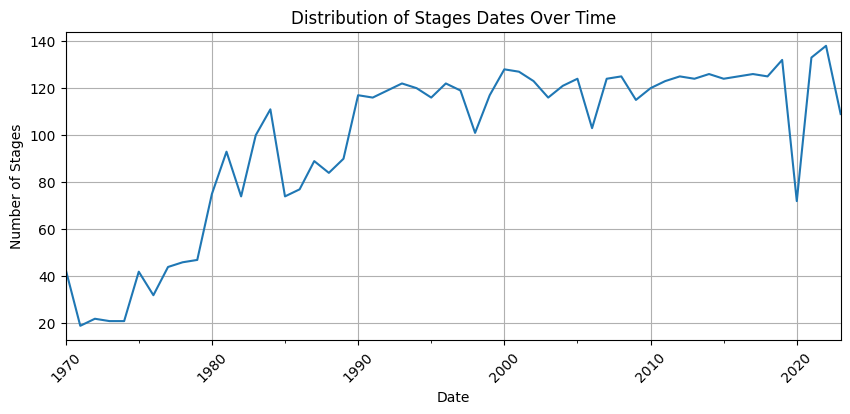
\includegraphics[width=0.5\linewidth]{images//DU/start_date_plot.png}
    \caption{\small Stages frequency per year plot}
    \label{fig:start_date}
\end{figure}


\noindent \textbf{position}: it ranges from zero to the total number of participants minus one, with all values being valid and following a monotonically increasing order.\\

\noindent \textbf{cyclist}: it contains the unique identifiers for cyclists. We noticed 249 duplicate entries within the same stages, which will be addressed during the \autoref{sec: data_cleaning} phase. No null values are present.\\

\noindent \textbf{cyclist\_age}: this feature represents the age of cyclists in a specific stage. It includes 113 null entries, with ages ranging from 13 to 56 years and an overall average of 28 years. To avoid skewing caused by cyclists appearing in multiple stages, we analyzed the average cyclist age per stage. The average age ranges from a minimum of 23 to a maximum of 31 years. When visualizing the average age across stages (averaging over all stages in a given year), we observe an increasing trend in the average age over time.\\

\noindent \textbf{is\_tarmac}: this binary feature indicates whether the stage surface is tarmac or not. There are no missing values, and 19\% of the feature values are false for individual stages, with the same value being applied to all instances of a given stage. \\

\noindent \textbf{is\_cobbled}: this binary feature indicates whether the stage surface is tarmac or not. All values are set to false, so the feature is unusable. \\

\noindent \textbf{is\_gravel}: this binary feature indicates whether the stage surface is gravel or not. All values are set to false, so the feature is unusable.\\

\noindent \textbf{cyclist\_team}: this alphanumeric feature represents the cyclist's team. A cyclist may have competed with different teams throughout their career.\\

\noindent \textbf{delta}: this numeric column represents the time difference between the current cyclist and the first-place finisher. We observed that it perfectly matches the duration column and contains $3'239$ non-increasing values with also some wrong negative values. As a result, we decided not to use this feature and instead focus the analysis on stage winners.\\

\noindent
\textbf{Null Values}\\
As for cycling datasets, we reported the heat map of null values in \autoref{fig:raes_heatmap}, to better visualize null values in the dataset.

\begin{figure}[H]
    \centering
    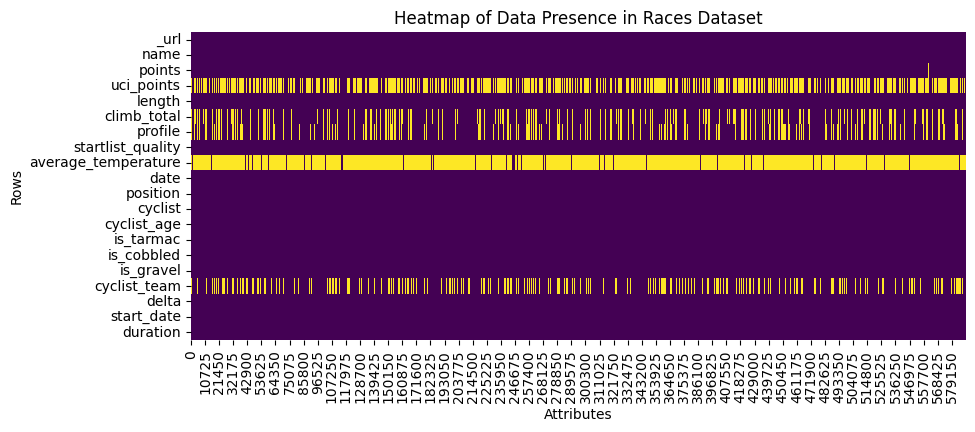
\includegraphics[width=0.6\linewidth]{images//DU/heatmap_races.png}
    \caption{\small Races null values heat-map}
    \label{fig:raes_heatmap}
\end{figure}


\noindent
\textbf{Correlations}\\
The only features with a slightly higher correlation are \textit{profile} and \textit{climb\_total} as races with a higher profile (such as mountainous or high-mountainous races) typically involve a greater number of kilometers climbed.\\

\begin{center}
    \begin{figure}[H]
    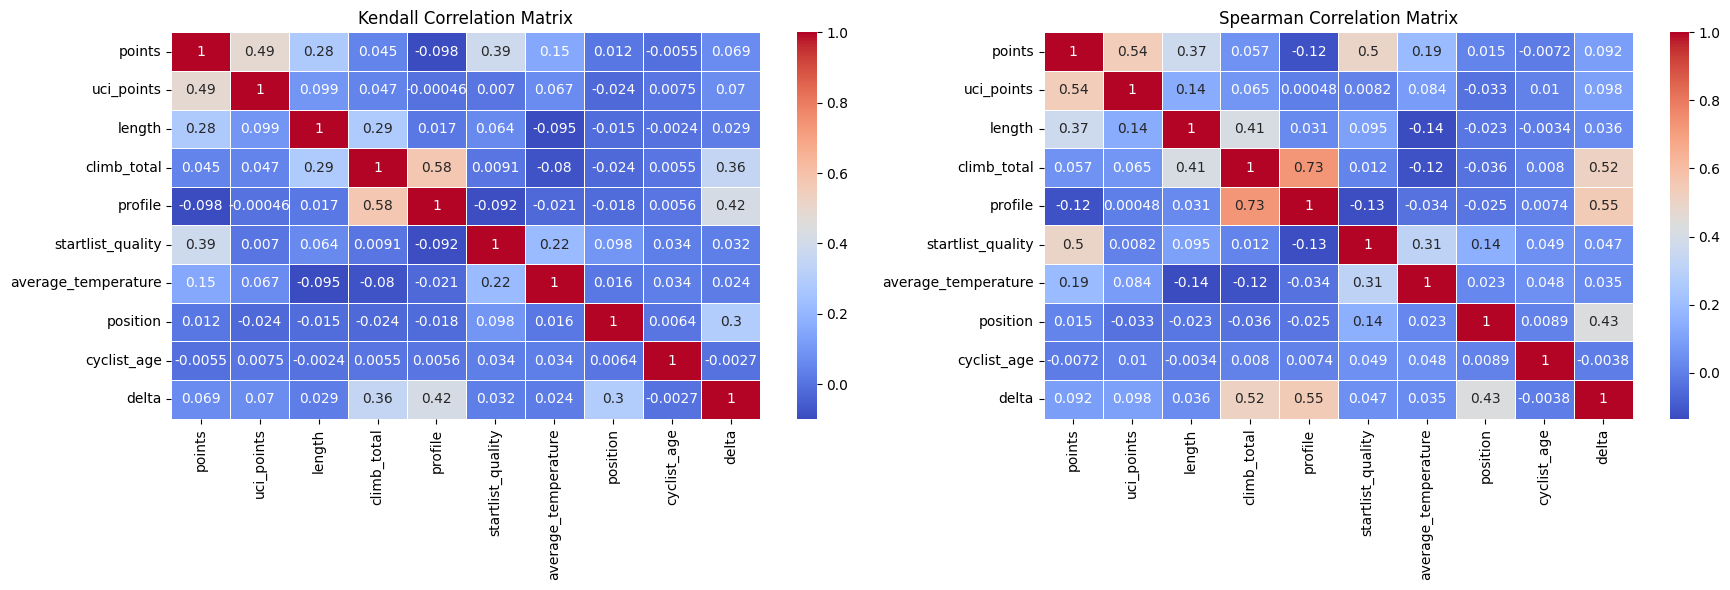
\includegraphics[width=0.9\textwidth]{images/DU/races_corr.png}
    \caption{Correlation between numerical features in races dataset}
    \end{figure}
\end{center}

\vspace{-1.2cm}
\noindent
\textbf{Consistency and issues}\\
A check was conducted to verify whether all features, whose values are replicated across all rows for a given stage were consistent in their copies. For example, the length should remain the same for all copies within a specific stage and all features were found to be consistent. \\
The main issues identified in the dataset are the following:

\begin{itemize}
    \item \textbf{Race terrain features:} The categorical boolean features \textit{is\_cobbled} and \textit{is\_gravel} are always false, unlike \textit{is\_tarmac}. As a result, whenever \textit{is\_tarmac} is false, the other two features do not provide any useful information.
    \item \textbf{Incorrect delta values:} This value represents the time difference between a cyclist and the race winner. However, in many races this value is negative, making it meaningless. We also attempted to calculate these values by checking the start and finish times of the races, but we found that they were consistent with the reported delta values. We observed several cases where cyclists in position $m$ had a total time lower than cyclists in position $n$, where $m > n$. This is logically impossible and further confirms the inconsistencies in the data.
    \item \textbf{Duplicated cyclists:} There are stages where a cyclist appears multiple times in different positions.
\end{itemize}


% -------------- Both dataset ------------------


\subsection{Races and Cyclists dataset}
Comparing the two datasets, it was confirmed that every cyclist who has competed is included in the cyclist's dataset. Instead, the opposite was found: there are about ten cyclists who have never participated in any race (according to our data).\\

\noindent
In the notebook \texttt{'TASK\_1/data\_understanding.ipynb'}, one can find all the details for each feature of both datasets, including distributions and box plots.\\






